% Options for packages loaded elsewhere
\PassOptionsToPackage{unicode}{hyperref}
\PassOptionsToPackage{hyphens}{url}
\documentclass[
  10pt,
]{article}
\usepackage{xcolor}
\usepackage[left=2cm, right=2cm, top=2cm, bottom=2cm]{geometry}
\usepackage{amsmath,amssymb}
\setcounter{secnumdepth}{-\maxdimen} % remove section numbering
\usepackage{iftex}
\ifPDFTeX
  \usepackage[T1]{fontenc}
  \usepackage[utf8]{inputenc}
  \usepackage{textcomp} % provide euro and other symbols
\else % if luatex or xetex
  \usepackage{unicode-math} % this also loads fontspec
  \defaultfontfeatures{Scale=MatchLowercase}
  \defaultfontfeatures[\rmfamily]{Ligatures=TeX,Scale=1}
\fi
\usepackage{lmodern}
\ifPDFTeX\else
  % xetex/luatex font selection
\fi
% Use upquote if available, for straight quotes in verbatim environments
\IfFileExists{upquote.sty}{\usepackage{upquote}}{}
\IfFileExists{microtype.sty}{% use microtype if available
  \usepackage[]{microtype}
  \UseMicrotypeSet[protrusion]{basicmath} % disable protrusion for tt fonts
}{}
\makeatletter
\@ifundefined{KOMAClassName}{% if non-KOMA class
  \IfFileExists{parskip.sty}{%
    \usepackage{parskip}
  }{% else
    \setlength{\parindent}{0pt}
    \setlength{\parskip}{6pt plus 2pt minus 1pt}}
}{% if KOMA class
  \KOMAoptions{parskip=half}}
\makeatother
\usepackage{color}
\usepackage{fancyvrb}
\newcommand{\VerbBar}{|}
\newcommand{\VERB}{\Verb[commandchars=\\\{\}]}
\DefineVerbatimEnvironment{Highlighting}{Verbatim}{commandchars=\\\{\}}
% Add ',fontsize=\small' for more characters per line
\usepackage{framed}
\definecolor{shadecolor}{RGB}{248,248,248}
\newenvironment{Shaded}{\begin{snugshade}}{\end{snugshade}}
\newcommand{\AlertTok}[1]{\textcolor[rgb]{0.94,0.16,0.16}{#1}}
\newcommand{\AnnotationTok}[1]{\textcolor[rgb]{0.56,0.35,0.01}{\textbf{\textit{#1}}}}
\newcommand{\AttributeTok}[1]{\textcolor[rgb]{0.13,0.29,0.53}{#1}}
\newcommand{\BaseNTok}[1]{\textcolor[rgb]{0.00,0.00,0.81}{#1}}
\newcommand{\BuiltInTok}[1]{#1}
\newcommand{\CharTok}[1]{\textcolor[rgb]{0.31,0.60,0.02}{#1}}
\newcommand{\CommentTok}[1]{\textcolor[rgb]{0.56,0.35,0.01}{\textit{#1}}}
\newcommand{\CommentVarTok}[1]{\textcolor[rgb]{0.56,0.35,0.01}{\textbf{\textit{#1}}}}
\newcommand{\ConstantTok}[1]{\textcolor[rgb]{0.56,0.35,0.01}{#1}}
\newcommand{\ControlFlowTok}[1]{\textcolor[rgb]{0.13,0.29,0.53}{\textbf{#1}}}
\newcommand{\DataTypeTok}[1]{\textcolor[rgb]{0.13,0.29,0.53}{#1}}
\newcommand{\DecValTok}[1]{\textcolor[rgb]{0.00,0.00,0.81}{#1}}
\newcommand{\DocumentationTok}[1]{\textcolor[rgb]{0.56,0.35,0.01}{\textbf{\textit{#1}}}}
\newcommand{\ErrorTok}[1]{\textcolor[rgb]{0.64,0.00,0.00}{\textbf{#1}}}
\newcommand{\ExtensionTok}[1]{#1}
\newcommand{\FloatTok}[1]{\textcolor[rgb]{0.00,0.00,0.81}{#1}}
\newcommand{\FunctionTok}[1]{\textcolor[rgb]{0.13,0.29,0.53}{\textbf{#1}}}
\newcommand{\ImportTok}[1]{#1}
\newcommand{\InformationTok}[1]{\textcolor[rgb]{0.56,0.35,0.01}{\textbf{\textit{#1}}}}
\newcommand{\KeywordTok}[1]{\textcolor[rgb]{0.13,0.29,0.53}{\textbf{#1}}}
\newcommand{\NormalTok}[1]{#1}
\newcommand{\OperatorTok}[1]{\textcolor[rgb]{0.81,0.36,0.00}{\textbf{#1}}}
\newcommand{\OtherTok}[1]{\textcolor[rgb]{0.56,0.35,0.01}{#1}}
\newcommand{\PreprocessorTok}[1]{\textcolor[rgb]{0.56,0.35,0.01}{\textit{#1}}}
\newcommand{\RegionMarkerTok}[1]{#1}
\newcommand{\SpecialCharTok}[1]{\textcolor[rgb]{0.81,0.36,0.00}{\textbf{#1}}}
\newcommand{\SpecialStringTok}[1]{\textcolor[rgb]{0.31,0.60,0.02}{#1}}
\newcommand{\StringTok}[1]{\textcolor[rgb]{0.31,0.60,0.02}{#1}}
\newcommand{\VariableTok}[1]{\textcolor[rgb]{0.00,0.00,0.00}{#1}}
\newcommand{\VerbatimStringTok}[1]{\textcolor[rgb]{0.31,0.60,0.02}{#1}}
\newcommand{\WarningTok}[1]{\textcolor[rgb]{0.56,0.35,0.01}{\textbf{\textit{#1}}}}
\usepackage{graphicx}
\makeatletter
\newsavebox\pandoc@box
\newcommand*\pandocbounded[1]{% scales image to fit in text height/width
  \sbox\pandoc@box{#1}%
  \Gscale@div\@tempa{\textheight}{\dimexpr\ht\pandoc@box+\dp\pandoc@box\relax}%
  \Gscale@div\@tempb{\linewidth}{\wd\pandoc@box}%
  \ifdim\@tempb\p@<\@tempa\p@\let\@tempa\@tempb\fi% select the smaller of both
  \ifdim\@tempa\p@<\p@\scalebox{\@tempa}{\usebox\pandoc@box}%
  \else\usebox{\pandoc@box}%
  \fi%
}
% Set default figure placement to htbp
\def\fps@figure{htbp}
\makeatother
\setlength{\emergencystretch}{3em} % prevent overfull lines
\providecommand{\tightlist}{%
  \setlength{\itemsep}{0pt}\setlength{\parskip}{0pt}}
\usepackage{microtype}
\usepackage{fvextra}
\DefineVerbatimEnvironment{Highlighting}{Verbatim}{breaklines,commandchars=\\\{\}}
\sloppy
\usepackage{longtable}
\usepackage{fvextra}
\usepackage{bookmark}
\IfFileExists{xurl.sty}{\usepackage{xurl}}{} % add URL line breaks if available
\urlstyle{same}
\hypersetup{
  pdftitle={GROUP WORK},
  pdfauthor={ALPHA NUMERIC},
  hidelinks,
  pdfcreator={LaTeX via pandoc}}

\title{GROUP WORK}
\author{ALPHA NUMERIC}
\date{2026-03-24}

\begin{document}
\maketitle

We proceeded to load marketing data from the `datarium' library.\\

\begin{Shaded}
\begin{Highlighting}[]
\FunctionTok{data}\NormalTok{(}\StringTok{"marketing"}\NormalTok{, }\AttributeTok{package =} \StringTok{"datarium"}\NormalTok{)}
\FunctionTok{head}\NormalTok{(marketing)}
\end{Highlighting}
\end{Shaded}

\begin{verbatim}
#>   youtube facebook newspaper sales
#> 1  276.12    45.36     83.04 26.52
#> 2   53.40    47.16     54.12 12.48
#> 3   20.64    55.08     83.16 11.16
#> 4  181.80    49.56     70.20 22.20
#> 5  216.96    12.96     70.08 15.48
#> 6   10.44    58.68     90.00  8.64
\end{verbatim}

Checking the names of the columns and some summary statistics.\\

\begin{Shaded}
\begin{Highlighting}[]
\FunctionTok{names}\NormalTok{(marketing)}
\end{Highlighting}
\end{Shaded}

\begin{verbatim}
#> [1] "youtube"   "facebook"  "newspaper" "sales"
\end{verbatim}

\begin{Shaded}
\begin{Highlighting}[]
\FunctionTok{dim}\NormalTok{(marketing)}
\end{Highlighting}
\end{Shaded}

\begin{verbatim}
#> [1] 200   4
\end{verbatim}

\begin{Shaded}
\begin{Highlighting}[]
\FunctionTok{summary}\NormalTok{(marketing)}
\end{Highlighting}
\end{Shaded}

\begin{verbatim}
#>     youtube          facebook       newspaper     
#>  Min.   :  0.84   Min.   : 0.00   Min.   :  0.36  
#>  1st Qu.: 89.25   1st Qu.:11.97   1st Qu.: 15.30  
#>  Median :179.70   Median :27.48   Median : 30.90  
#>  Mean   :176.45   Mean   :27.92   Mean   : 36.66  
#>  3rd Qu.:262.59   3rd Qu.:43.83   3rd Qu.: 54.12  
#>  Max.   :355.68   Max.   :59.52   Max.   :136.80  
#>      sales      
#>  Min.   : 1.92  
#>  1st Qu.:12.45  
#>  Median :15.48  
#>  Mean   :16.83  
#>  3rd Qu.:20.88  
#>  Max.   :32.40
\end{verbatim}

From the summary statistics, we were able to have a glimpse of our
marketing dataset. It was evident that more budget was allocated to
YouTube (176.45), than the rest of the marketing channels.\\
We proceeded to investigate if our linear model assumptions were
violated. We began with the most prominent one which is the
\textbf{Assumption of Normality}.\\

\subsection{Assumption of Normality
checks}\label{assumption-of-normality-checks}

From our data, it was evident that our dependent variable was
\emph{sales} as our independent variables were \emph{YouTube},
\emph{Facebook} and \emph{News Paper}.\\
We began by use of a histogram. For the bin-width the range (Max - Min)
from our summary statistics guided us.\\

\begin{Shaded}
\begin{Highlighting}[]
\FunctionTok{ggplot}\NormalTok{(marketing, }\FunctionTok{aes}\NormalTok{(}\AttributeTok{x =}\NormalTok{ youtube)) }\SpecialCharTok{+} \FunctionTok{geom\_histogram}\NormalTok{(}\AttributeTok{binwidth =} \DecValTok{20}\NormalTok{,}
    \AttributeTok{fill =} \StringTok{"blue"}\NormalTok{, }\AttributeTok{color =} \StringTok{"black"}\NormalTok{) }\SpecialCharTok{+} \FunctionTok{labs}\NormalTok{(}\AttributeTok{title =} \StringTok{"Histogram of YouTube"}\NormalTok{,}
    \AttributeTok{x =} \StringTok{"YouTube"}\NormalTok{, }\AttributeTok{y =} \StringTok{"Count"}\NormalTok{)}
\end{Highlighting}
\end{Shaded}

\begin{center}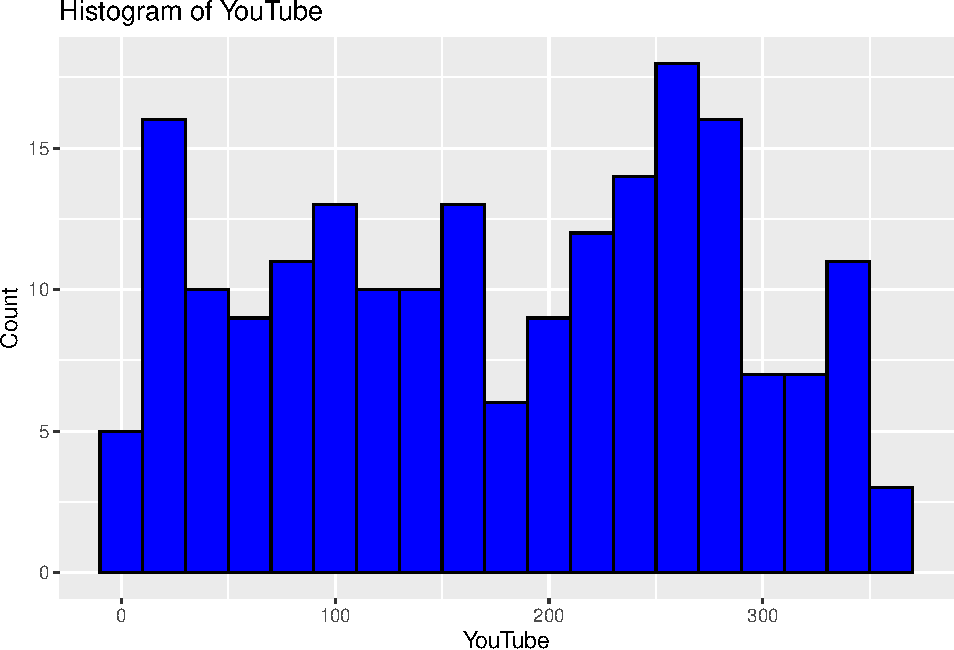
\includegraphics{Marketing_datarium_files/figure-latex/YouTube-1} \end{center}

The YouTube Histogram appeared to be bi-modal.\\

\begin{Shaded}
\begin{Highlighting}[]
\FunctionTok{ggplot}\NormalTok{(marketing, }\FunctionTok{aes}\NormalTok{(}\AttributeTok{x =}\NormalTok{ facebook)) }\SpecialCharTok{+} \FunctionTok{geom\_histogram}\NormalTok{(}\AttributeTok{binwidth =} \DecValTok{5}\NormalTok{,}
    \AttributeTok{fill =} \StringTok{"purple"}\NormalTok{, }\AttributeTok{color =} \StringTok{"black"}\NormalTok{) }\SpecialCharTok{+} \FunctionTok{labs}\NormalTok{(}\AttributeTok{title =} \StringTok{"Histogram of Facebook"}\NormalTok{,}
    \AttributeTok{x =} \StringTok{"Facebook"}\NormalTok{, }\AttributeTok{y =} \StringTok{"Count"}\NormalTok{)}
\end{Highlighting}
\end{Shaded}

\begin{center}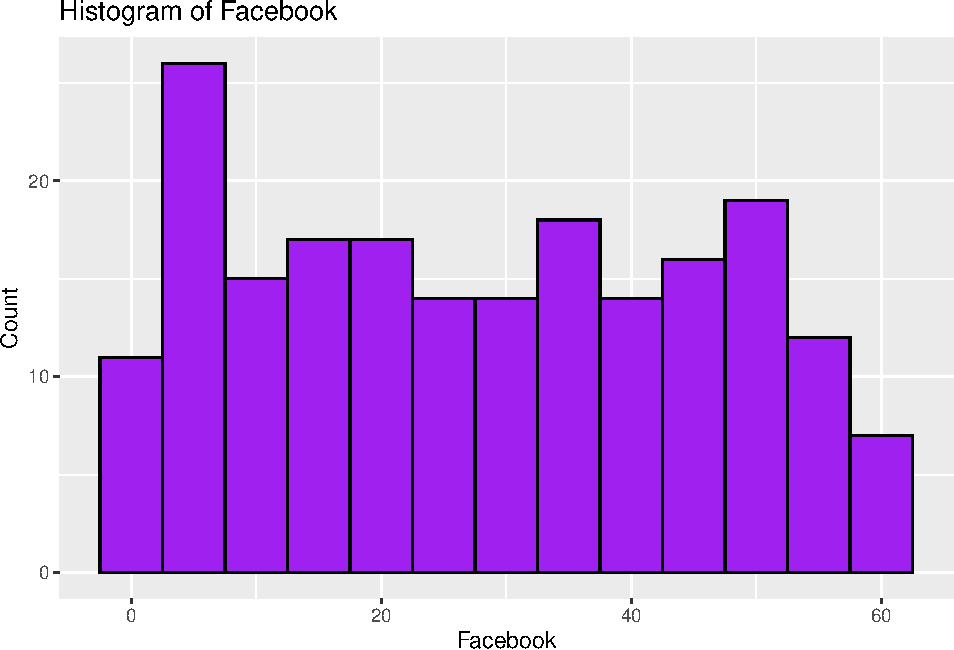
\includegraphics{Marketing_datarium_files/figure-latex/Facebook-1} \end{center}

The histogram was uni-modal and appeared to be mesokurtic.\\

\begin{Shaded}
\begin{Highlighting}[]
\FunctionTok{ggplot}\NormalTok{(marketing, }\FunctionTok{aes}\NormalTok{(}\AttributeTok{x =}\NormalTok{ newspaper)) }\SpecialCharTok{+} \FunctionTok{geom\_histogram}\NormalTok{(}\AttributeTok{binwidth =} \DecValTok{10}\NormalTok{,}
    \AttributeTok{fill =} \StringTok{"gold"}\NormalTok{, }\AttributeTok{color =} \StringTok{"black"}\NormalTok{) }\SpecialCharTok{+} \FunctionTok{labs}\NormalTok{(}\AttributeTok{title =} \StringTok{"Histogram of Newspaper"}\NormalTok{,}
    \AttributeTok{x =} \StringTok{"Newspaper"}\NormalTok{, }\AttributeTok{y =} \StringTok{"Count"}\NormalTok{)}
\end{Highlighting}
\end{Shaded}

\begin{center}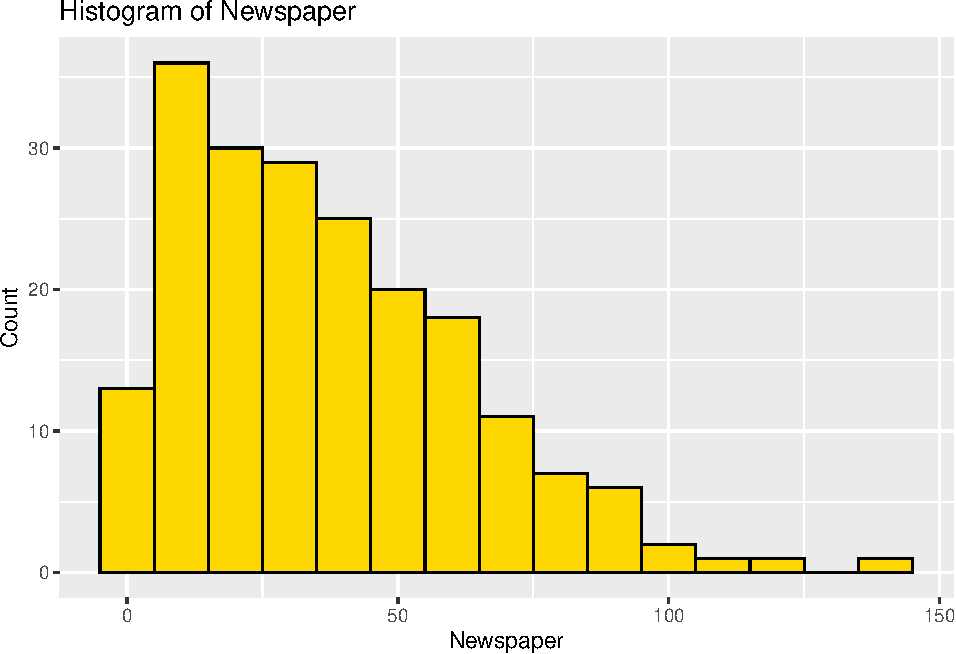
\includegraphics{Marketing_datarium_files/figure-latex/newspaper-1} \end{center}

The histogram was positively skewed as it had a longer tail towards the
right.\\

\begin{Shaded}
\begin{Highlighting}[]
\FunctionTok{ggplot}\NormalTok{(marketing, }\FunctionTok{aes}\NormalTok{(}\AttributeTok{x =}\NormalTok{ sales)) }\SpecialCharTok{+} \FunctionTok{geom\_histogram}\NormalTok{(}\AttributeTok{binwidth =} \DecValTok{3}\NormalTok{,}
    \AttributeTok{fill =} \StringTok{"red"}\NormalTok{, }\AttributeTok{color =} \StringTok{"black"}\NormalTok{) }\SpecialCharTok{+} \FunctionTok{labs}\NormalTok{(}\AttributeTok{title =} \StringTok{"Histogram of Sales"}\NormalTok{,}
    \AttributeTok{x =} \StringTok{"Sales"}\NormalTok{, }\AttributeTok{y =} \StringTok{"Count"}\NormalTok{)}
\end{Highlighting}
\end{Shaded}

\begin{center}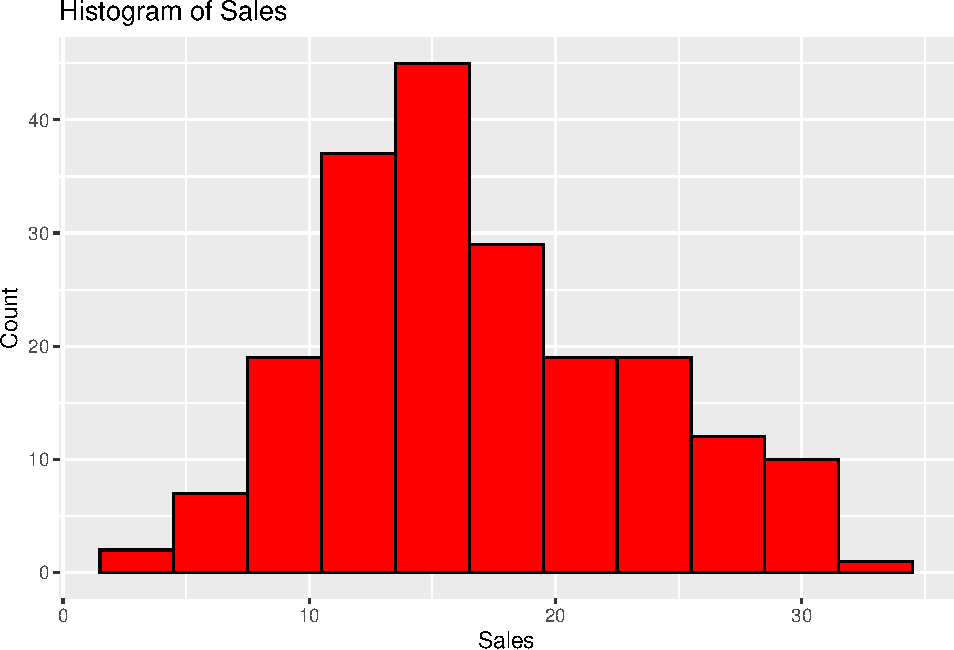
\includegraphics{Marketing_datarium_files/figure-latex/sales-1} \end{center}

The histogram appeared to be almost normally distributed.

\end{document}
